\documentclass[12pt,a4paper]{article}

\usepackage[T1]{fontenc}
\usepackage[utf8]{inputenc}
\usepackage[brazil]{babel}
\usepackage{newtxtext,newtxmath}
\usepackage{microtype}
\usepackage{geometry}
\usepackage{setspace}
\usepackage{enumitem}
\usepackage{xcolor}
\usepackage{graphicx}
\usepackage[colorlinks=true,citecolor=blue,linkcolor=black,urlcolor=blue]{hyperref}

\geometry{margin=2.5cm}
\setstretch{1.15}
\setlength{\parindent}{1.25cm}
\setlength{\parskip}{0pt}

\begin{document}

\begin{center}
  \textbf{INSTITUTO BRASILEIRO DE ENSINO, DESENVOLVIMENTO E PESQUISA (IDP)}\par
  \textbf{CURSO DE ADMINISTRAÇÃO PÚBLICA}\par
  \vspace{1.8em}
  {\Large\bfseries Análise crítica de uma representação gráfica enganosa nas eleições de 2026\par}
  \vspace{0.6em}
  {\large Pesquisa eleitoral AtlasIntel/Bloomberg e a circulação de uma imagem com dados adulterados\par}
  \vspace{1.8em}
  Fabricio Fernandes Santana
\end{center}



\section{Material selecionado}

O material analisado é uma imagem que circulou no Facebook, no X, no YouTube e
no Instagram com a afirmação: ``Pesquisa barrada por Nunes Marques --- 75\%
Lula contra 25\% Flávio Bolsonaro''. A imagem pode ser consultada na
\href{https://noticias.uol.com.br/confere/ultimas-noticias/2026/06/12/lula-nao-teve-75-de-intencoes-de-voto-em-pesquisa-suspensa-pelo-tse.ghtm}{reprodução publicada pelo UOL Confere}.

\begin{figure}[htbp]
  \centering
  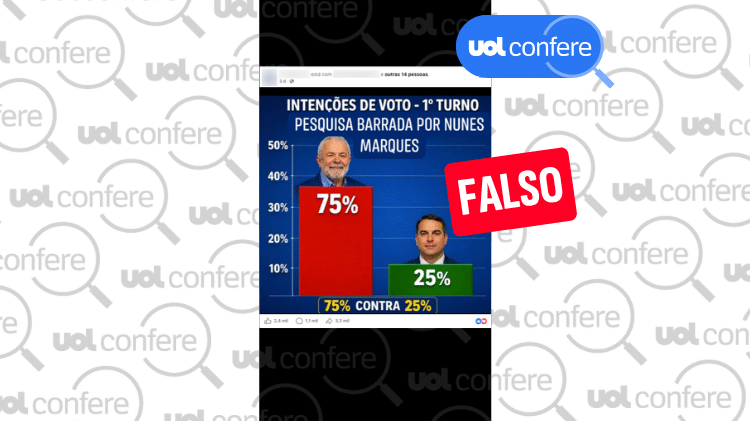
\includegraphics[width=\linewidth]{figuras/lula.png}
  \caption{Imagem viral analisada na atividade.}
  \par\smallskip
  {\small\textbf{Fonte:} reprodução da publicação viral, conforme registro do UOL Confere.}
\end{figure}

A imagem foi publicada e compartilhada antes de ser checada por veículos de
verificação. A checagem do UOL Confere foi publicada em 12 de junho de 2026.
A pesquisa à qual a imagem se referia era a AtlasIntel/Bloomberg, divulgada em
19 de maio de 2026 e registrada no Tribunal Superior Eleitoral sob o número
BR-06939/2026.

\section{Contextualização}

O gráfico pretende apresentar um cenário de primeiro turno da eleição
presidencial de 2026, sugerindo uma vantagem muito ampla de Luiz Inácio Lula da
Silva sobre Flávio Bolsonaro: 75\% contra 25\%. A referência à suspensão da
pesquisa pelo ministro Nunes Marques procura conferir aparência de autenticidade
e relevância institucional à imagem.

O relatório original, entretanto, registrou Lula com 47\% e Flávio Bolsonaro
com 34,3\% nesse cenário. A pesquisa ouviu 5.032 respondentes entre 13 e 18 de
maio de 2026, com margem de erro de 1 ponto percentual e nível de confiança de
95\%.

\section{Análise crítica}

A representação é enganosa por dois motivos principais.

Primeiro, os números escritos sobre o gráfico não correspondem ao levantamento
ao qual ele é atribuído. A diferença entre os candidatos na pesquisa original
era de 12,7 pontos percentuais, e não de 50 pontos. Portanto, não se trata
apenas de uma escolha estética de escala: os valores foram alterados.

Segundo, há uma incompatibilidade visual entre as barras e os rótulos. A barra
de Lula aparece aproximadamente na faixa de 30\% a 40\% do eixo, e a de Flávio
próxima de 10\%, embora os textos indiquem 75\% e 25\%. Um leitor que observa a
imagem rapidamente pode confiar nos números destacados e na aparência de um
gráfico de pesquisa sem verificar a escala.

A peça também omite informações essenciais para a leitura: instituto, tamanho
da amostra, período da coleta, margem de erro, cenário testado, demais
candidatos e respostas como branco, nulo e não sabe. A menção à suspensão pelo
TSE aparece sem esclarecer que a decisão tratava da divulgação da pesquisa e de
questionamentos metodológicos; ela não transformava os percentuais em 75\% e
25\%.

O problema não depende da posição política de quem publicou. Ele está na
combinação entre atribuição de fonte, números incompatíveis, escala visual
inconsistente e ausência de contexto metodológico. Esses recursos podem levar
o público a interpretar uma vantagem de 12,7 pontos como se fosse uma diferença
de 50 pontos.

\section{Proposta de correção}

Eu substituiria a imagem por um gráfico de barras horizontais, com o eixo
iniciado em zero e uma escala comum até 100\%. As barras deveriam apresentar os
valores efetivamente publicados na pesquisa: Lula com 47,0\% e Flávio Bolsonaro
com 34,3\%, além dos demais candidatos e das categorias de resposta disponíveis.

Abaixo do gráfico, incluiria a seguinte nota metodológica:

\begin{quote}
\small
AtlasIntel/Bloomberg; 5.032 respondentes; coleta de 13 a 18/05/2026; margem de
erro de $\pm$1 ponto percentual; confiança de 95\%; registro TSE
BR-06939/2026. Trata-se de intenção de voto estimulada em um cenário hipotético
de primeiro turno, e não de previsão do resultado eleitoral.
\end{quote}

Se o objetivo fosse destacar a diferença, ela poderia ser indicada por uma
anotação de 12,7 pontos percentuais, nunca por uma barra ou rótulo que sugerisse
50 pontos. A fonte completa e um link para o relatório original permitiriam a
conferência independente dos dados.

\section{Fontes consultadas}

\begin{itemize}
  \item UOL Confere. \textit{Lula obteve 47\%, e não 75\% em pesquisa eleitoral suspensa por Nunes Marques}. Publicado em 12 jun. 2026. Disponível em: \href{https://noticias.uol.com.br/confere/ultimas-noticias/2026/06/12/lula-nao-teve-75-de-intencoes-de-voto-em-pesquisa-suspensa-pelo-tse.ghtm}{UOL Confere}. Acesso em: 19 set. 2026.
  \item ATLASINTEL/BLOOMBERG. \textit{Pesquisa Atlas/Bloomberg --- maio 2026}. Disponível em: \href{https://cdn.bncamazonas.com.br/wp-content/uploads/2026/05/AtlasIntel-19maio2026.pdf}{relatório original}. Acesso em: 19 set. 2026.
  \item AGÊNCIA LUPA. \textit{É falso que pesquisa AtlasIntel suspensa pelo TSE apontou 75\% para Lula no 1º turno}. Publicado em 12 jun. 2026. Disponível em: \href{https://www.agencialupa.org/verificacao/2026/06/12/e-falso-que-pesquisa-atlasintel-suspensa-pelo-tse-apontou-75-para-lula-no-1-turno/}{Agência Lupa}. Acesso em: 19 set. 2026.
  \item TRIBUNAL SUPERIOR ELEITORAL. \textit{TSE suspende divulgação de pesquisa da AtlasIntel sobre disputa para presidente por suspeita de indução ao eleitor}. Disponível em: \href{https://www.tse.jus.br/comunicacao/noticias/2026/Junho/tse-suspende-divulgacao-de-pesquisa-da-atlasintel-sobre-disputa-para-presidente-por-suspeita-de-inducao-ao-eleitor}{TSE}. Acesso em: 19 set. 2026.
\end{itemize}


\end{document}
